\subsection{Challenges}
To finalize the overview and basics of data science, let's look at the typical challenges.

First, we have the challenge of \textbf{finding data}. There may be hundreds or thousands of tables, for example in the case of SAP the numbers can easily for up to $800'000$. But, different entities differ in their relevance, meaning some are less relevant than others.

The next challenge is the \textbf{transformation of data}, meaning reorganization of data, filtering, extraction of relevant features, and so on. Not only for transformations, but also in general other challenges are \textbf{dealing with big data and streaming data}. The challenge of big data evolved over the last few decades, meaning typical stochastic methods try to solve the problem of saying something about entities given only a small amount of samples, whereas now we have a very high load of data, and need to solve the problem of dealing with these large amounts in a correct way. Also for streaming data, new approaches need to be thought of. Additionally, we also need to \textbf{deal with a concept shift}.

Another huge challenge is ensuring \textbf{data quality}. This goes especially, since our provided data may be incomplete, invalid, inconsistent, imprecise, and/or outdated. Consider for example timestamps. They might be incomplete {\color{gray}\footnotesize(event is missing)}, invalid {\color{gray}\footnotesize(e.g. 14-14-2018)}, inconsistent {\color{gray}\footnotesize(14-07-2018 in contrast to 7-14-2018)}, or imprecise {\color{gray}\footnotesize(only regard part of available data: 2018-09-21\textit{\st{'T'13:00:10}})}.

A very typical problem is \textbf{overfitting and underfitting} as it can be seen \ref{fig:1_over_under_fitting}.

\begin{figure}[H]
  \centering
  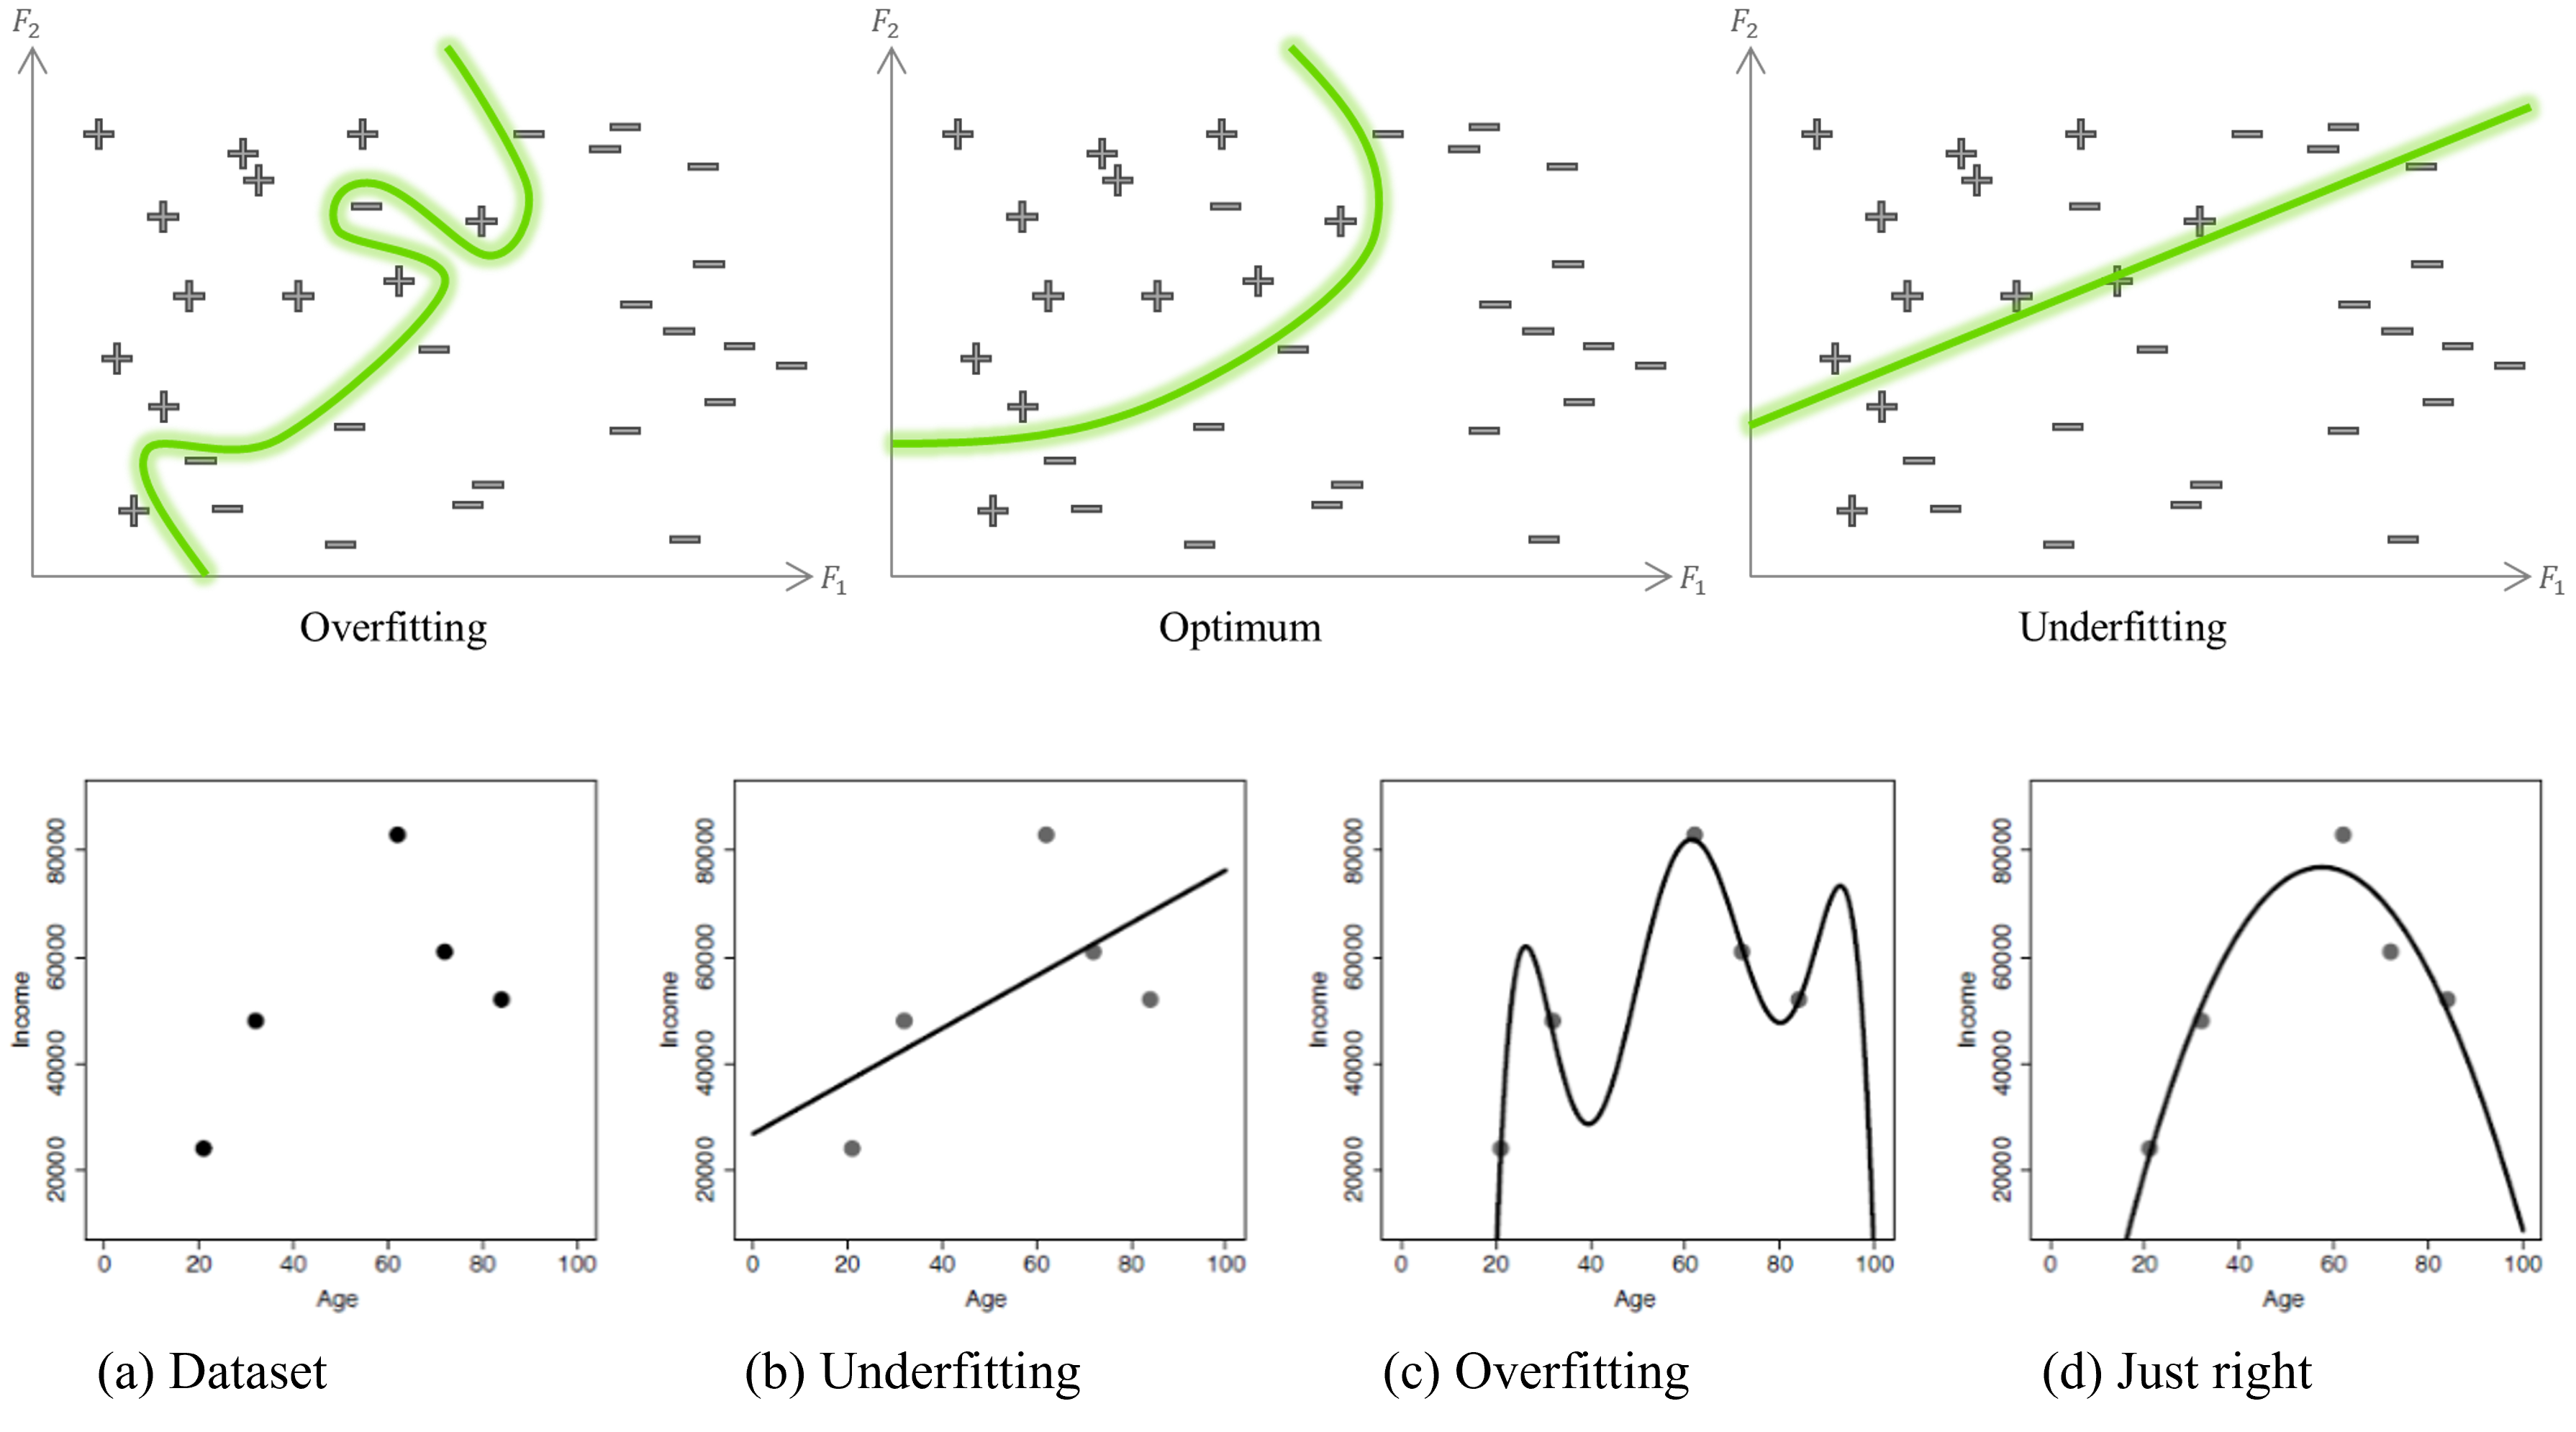
\includegraphics[width=0.9\textwidth]{assets/basics/over_under_fitting.png}
  \caption{Over- and underfitting visualized}
  \label{fig:1_over_under_fitting}
\end{figure}

The next challenge is the distinction of \textbf{correlation and causation}, explicitly that correlation does not imply causation. Consider this example:
\begin{itemize}
  \item Sunburn and ice cream have a strong correlation. When only these two features are considered, one might derive that either ice cream causes sunburn, or the other way around.
  \item We know of course, that this is not correct and instead an additional factor causes both phenomena: if the sun is shining, it's warm and people eat ice cream, and also sun directly causes sunburn.
\end{itemize}

Besides the accuracy of our results, we also need to look into whether our results are valuable. Concretely, \textbf{results} should be \textbf{made actionable}. This means, that analysis results should be relevant, specific, timely, novel, and clear. Our goal is to go from "data" to "insight" and finally "action". Consider these examples:
\begin{itemize}
  \item Warning about a traffic jam should come before entering said traffic jam.
  \item That it's currently raining is not too helpful information. Preferably is a notice ahead of time.
\end{itemize}

The last, but very important challenge is \textbf{responsible data science} (RDS)\sidenote{Responsible data science}. This includes ensuring of:
\begin{itemize}
  \item \textbf{Fairness}, meaning data science should exclude prejudice {\color{gray}\footnotesize(How to avoid unfair conclusions even if they are true?)}
  \item \textbf{Accuracy}, so data science without guesswork {\color{gray}\footnotesize(How to answer questions with a guaranteed level of accuracy?)}
  \item \textbf{Confidentiality} {\color{gray}\footnotesize(How to answer questions without revealing secrets?)}
  \item \textbf{Transparency} {\color{gray}\footnotesize(How to clarify answers such that they become indisputable?)}
\end{itemize}